%%%%%%%%%%%%%%%%%%%%%%%%%%%%%%%%%%%%%%%%%
%  My documentation report
%  Objetive: Explain what I did and how, so someone can continue with the investigation
%
% Important note:
% Chapter heading images should have a 2:1 width:height ratio,
% e.g. 920px width and 460px height.
%
%%%%%%%%%%%%%%%%%%%%%%%%%%%%%%%%%%%%%%%%%

%----------------------------------------------------------------------------------------
%	PACKAGES AND OTHER DOCUMENT CONFIGURATIONS
%----------------------------------------------------------------------------------------

\documentclass[11pt,fleqn]{book} % Default font size and left-justified equations

\usepackage[top=2.5cm,bottom=2.5cm,left=3.2cm,right=3.2cm,headsep=10pt,letterpaper]{geometry} % Page margins

\usepackage{xcolor,lipsum} % Required for specifying colors by name
\definecolor{ocre}{RGB}{0,0,175} 
\definecolor{lightgray}{RGB}{229,229,229} 
% Font Settings
\usepackage{avant} % Use the Avantgarde font for headings
%\usepackage{times} % Use the Times font for headings
\usepackage{mathptmx} % Use the Adobe Times Roman as the default text font together with math symbols from the Sym­bol, Chancery and Com­puter Modern fonts

\usepackage{microtype} % Slightly tweak font spacing for aesthetics
\usepackage[utf8]{inputenc} % Required for including letters with accents
\usepackage[T1]{fontenc} % Use 8-bit encoding that has 256 glyphs


% MATHS PACKAGE
\usepackage{amsmath,tikz}
\usetikzlibrary{matrix}
\newcommand*{\horzbar}{\rule[0.05ex]{2.5ex}{0.5pt}}
\usepackage{calc}

% VERBATIM PACKAGE
\usepackage{verbatim}

% Bibliography
\usepackage[style=alphabetic,sorting=nyt,sortcites=true,autopunct=true,babel=hyphen,hyperref=true,abbreviate=false,backref=true,backend=biber]{biblatex}
\addbibresource{bibliography.bib} % BibTeX bibliography file
\defbibheading{bibempty}{}

%----------------------------------------------------------------------------------------
%	VARIOUS REQUIRED PACKAGES
%----------------------------------------------------------------------------------------

\usepackage{titlesec} % Allows customization of titles

\usepackage{graphicx} % Required for including pictures
\graphicspath{{Pictures/}} % Specifies the directory where pictures are stored

\usepackage{lipsum} % Inserts dummy text

\usepackage{tikz} % Required for drawing custom shapes

\usepackage[english]{babel} % English language/hyphenation

\usepackage{enumitem} % Customize lists
\setlist{nolistsep} % Reduce spacing between bullet points and numbered lists

\usepackage{booktabs} % Required for nicer horizontal rules in tables

\usepackage{eso-pic} % Required for specifying an image background in the title page

%----------------------------------------------------------------------------------------
%	MAIN TABLE OF CONTENTS
%----------------------------------------------------------------------------------------

\usepackage{titletoc} % Required for manipulating the table of contents

\contentsmargin{0cm} % Removes the default margin
% Chapter text styling
\titlecontents{chapter}[1.25cm] % Indentation
{\addvspace{15pt}\large\sffamily\bfseries} % Spacing and font options for chapters
{\color{ocre!60}\contentslabel[\Large\thecontentslabel]{1.25cm}\color{ocre}} % Chapter number
{}  
{\color{ocre!60}\normalsize\sffamily\bfseries\;\titlerule*[.5pc]{.}\;\thecontentspage} % Page number
% Section text styling
\titlecontents{section}[1.25cm] % Indentation
{\addvspace{5pt}\sffamily\bfseries} % Spacing and font options for sections
{\contentslabel[\thecontentslabel]{1.25cm}} % Section number
{}
{\sffamily\hfill\color{black}\thecontentspage} % Page number
[]
% Subsection text styling
\titlecontents{subsection}[1.25cm] % Indentation
{\addvspace{1pt}\sffamily\small} % Spacing and font options for subsections
{\contentslabel[\thecontentslabel]{1.25cm}} % Subsection number
{}
{\sffamily\;\titlerule*[.5pc]{.}\;\thecontentspage} % Page number
[] 

%----------------------------------------------------------------------------------------
%	MINI TABLE OF CONTENTS IN CHAPTER HEADS
%----------------------------------------------------------------------------------------

% Section text styling
\titlecontents{lsection}[0em] % Indendating
{\footnotesize\sffamily} % Font settings
{}
{}
{}

% Subsection text styling
\titlecontents{lsubsection}[.5em] % Indentation
{\normalfont\footnotesize\sffamily} % Font settings
{}
{}
{}
 
%----------------------------------------------------------------------------------------
%	PAGE HEADERS
%----------------------------------------------------------------------------------------

\usepackage{fancyhdr} % Required for header and footer configuration

\pagestyle{fancy}
\renewcommand{\chaptermark}[1]{\markboth{\sffamily\normalsize\bfseries\chaptername\ \thechapter.\ #1}{}} % Chapter text font settings
\renewcommand{\sectionmark}[1]{\markright{\sffamily\normalsize\thesection\hspace{5pt}#1}{}} % Section text font settings
\fancyhf{} \fancyhead[LE,RO]{\sffamily\normalsize\thepage} % Font setting for the page number in the header
\fancyhead[LO]{\rightmark} % Print the nearest section name on the left side of odd pages
\fancyhead[RE]{\leftmark} % Print the current chapter name on the right side of even pages
\renewcommand{\headrulewidth}{0.5pt} % Width of the rule under the header
\addtolength{\headheight}{2.5pt} % Increase the spacing around the header slightly
\renewcommand{\footrulewidth}{0pt} % Removes the rule in the footer
\fancypagestyle{plain}{\fancyhead{}\renewcommand{\headrulewidth}{0pt}} % Style for when a plain pagestyle is specified

% Removes the header from odd empty pages at the end of chapters
\makeatletter
\renewcommand{\cleardoublepage}{
\clearpage\ifodd\c@page\else
\hbox{}
\vspace*{\fill}
\thispagestyle{empty}
\newpage
\fi}

%----------------------------------------------------------------------------------------
%	THEOREM STYLES
%----------------------------------------------------------------------------------------

\usepackage{amsmath,amsfonts,amssymb,amsthm} % For math equations, theorems, symbols, etc

\newcommand{\intoo}[2]{\mathopen{]}#1\,;#2\mathclose{[}}
\newcommand{\ud}{\mathop{\mathrm{{}d}}\mathopen{}}
\newcommand{\intff}[2]{\mathopen{[}#1\,;#2\mathclose{]}}
\newtheorem{notation}{Notation}[chapter]

%%%%%%%%%%%%%%%%%%%%%%%%%%%%%%%%%%%%%%%%%%%%%%%%%%%%%%%%%%%%%%%%%%%%%%%%%%%
%%%%%%%%%%%%%%%%%%%% dedicated to boxed/framed environements %%%%%%%%%%%%%%
%%%%%%%%%%%%%%%%%%%%%%%%%%%%%%%%%%%%%%%%%%%%%%%%%%%%%%%%%%%%%%%%%%%%%%%%%%%
\newtheoremstyle{ocrenumbox}% % Theorem style name
{0pt}% Space above
{0pt}% Space below
{\normalfont}% % Body font
{}% Indent amount
{\small\bf\sffamily\color{ocre}}% % Theorem head font
{\;}% Punctuation after theorem head
{0.25em}% Space after theorem head
{\small\sffamily\color{ocre}\thmname{#1}\nobreakspace\thmnumber{\@ifnotempty{#1}{}\@upn{#2}}% Theorem text (e.g. Theorem 2.1)
\thmnote{\nobreakspace\the\thm@notefont\sffamily\bfseries\color{black}---\nobreakspace#3.}} % Optional theorem note
\renewcommand{\qedsymbol}{$\blacksquare$}% Optional qed square

\newtheoremstyle{blacknumex}% Theorem style name
{5pt}% Space above
{5pt}% Space below
{\normalfont}% Body font
{} % Indent amount
{\small\bf\sffamily}% Theorem head font
{\;}% Punctuation after theorem head
{0.25em}% Space after theorem head
{\small\sffamily{\tiny\ensuremath{\blacksquare}}\nobreakspace\thmname{#1}\nobreakspace\thmnumber{\@ifnotempty{#1}{}\@upn{#2}}% Theorem text (e.g. Theorem 2.1)
\thmnote{\nobreakspace\the\thm@notefont\sffamily\bfseries---\nobreakspace#3.}}% Optional theorem note

\newtheoremstyle{blacknumbox} % Theorem style name
{0pt}% Space above
{0pt}% Space below
{\normalfont}% Body font
{}% Indent amount
{\small\bf\sffamily}% Theorem head font
{\;}% Punctuation after theorem head
{0.25em}% Space after theorem head
{\small\sffamily\thmname{#1}\nobreakspace\thmnumber{\@ifnotempty{#1}{}\@upn{#2}}% Theorem text (e.g. Theorem 2.1)
\thmnote{\nobreakspace\the\thm@notefont\sffamily\bfseries---\nobreakspace#3.}}% Optional theorem note

%%%%%%%%%%%%%%%%%%%%%%%%%%%%%%%%%%%%%%%%%%%%%%%%%%%%%%%%%%%%%%%%%%%%%%%%%%%
%%%%%%%%%%%%% dedicated to non-boxed/non-framed environements %%%%%%%%%%%%%
%%%%%%%%%%%%%%%%%%%%%%%%%%%%%%%%%%%%%%%%%%%%%%%%%%%%%%%%%%%%%%%%%%%%%%%%%%%
\newtheoremstyle{ocrenum}% % Theorem style name
{5pt}% Space above
{5pt}% Space below
{\normalfont}% % Body font
{}% Indent amount
{\small\bf\sffamily\color{ocre}}% % Theorem head font
{\;}% Punctuation after theorem head
{0.25em}% Space after theorem head
{\small\sffamily\color{ocre}\thmname{#1}\nobreakspace\thmnumber{\@ifnotempty{#1}{}\@upn{#2}}% Theorem text (e.g. Theorem 2.1)
\thmnote{\nobreakspace\the\thm@notefont\sffamily\bfseries\color{black}---\nobreakspace#3.}} % Optional theorem note
\renewcommand{\qedsymbol}{$\blacksquare$}% Optional qed square
\makeatother

% Defines the theorem text style for each type of theorem to one of the three styles above
\newcounter{dummy} 
\numberwithin{dummy}{section}
\theoremstyle{ocrenumbox}
\newtheorem{theoremeT}[dummy]{Theorem}
\newtheorem{problem}{Problem}[chapter]
\newtheorem{exerciseT}{Exercise}[chapter]
\theoremstyle{blacknumex}
\newtheorem{exampleT}{Example}[chapter]
\theoremstyle{blacknumbox}
\newtheorem{vocabulary}{Vocabulary}[chapter]
\newtheorem{definitionT}{Definition}[section]
\newtheorem{corollaryT}[dummy]{Corollary}
\theoremstyle{ocrenum}
\newtheorem{proposition}[dummy]{Proposition}

%----------------------------------------------------------------------------------------
%	DEFINITION OF COLORED BOXES
%----------------------------------------------------------------------------------------

\RequirePackage[framemethod=default]{mdframed} % Required for creating the theorem, definition, exercise and corollary boxes

% Theorem box
\newmdenv[skipabove=7pt,
skipbelow=7pt,
backgroundcolor=black!5,
linecolor=ocre,
innerleftmargin=5pt,
innerrightmargin=5pt,
innertopmargin=5pt,
leftmargin=0cm,
rightmargin=0cm,
innerbottommargin=5pt]{tBox}

% Exercise box	  
\newmdenv[skipabove=7pt,
skipbelow=7pt,
rightline=false,
leftline=true,
topline=false,
bottomline=false,
backgroundcolor=ocre!10,
linecolor=ocre,
innerleftmargin=5pt,
innerrightmargin=5pt,
innertopmargin=5pt,
innerbottommargin=5pt,
leftmargin=0cm,
rightmargin=0cm,
linewidth=4pt]{eBox}	

% Definition box
\newmdenv[skipabove=7pt,
skipbelow=7pt,
rightline=false,
leftline=true,
topline=false,
bottomline=false,
linecolor=ocre,
innerleftmargin=5pt,
innerrightmargin=5pt,
innertopmargin=0pt,
leftmargin=0cm,
rightmargin=0cm,
linewidth=4pt,
innerbottommargin=0pt]{dBox}	

% Corollary box
\newmdenv[skipabove=7pt,
skipbelow=7pt,
rightline=false,
leftline=true,
topline=false,
bottomline=false,
linecolor=gray,
backgroundcolor=black!5,
innerleftmargin=5pt,
innerrightmargin=5pt,
innertopmargin=5pt,
leftmargin=0cm,
rightmargin=0cm,
linewidth=4pt,
innerbottommargin=5pt]{cBox}

% Creates an environment for each type of theorem and assigns it a theorem text style from the "Theorem Styles" section above and a colored box from above
\newenvironment{theorem}{\begin{tBox}\begin{theoremeT}}{\end{theoremeT}\end{tBox}}
\newenvironment{exercise}{\begin{eBox}\begin{exerciseT}}{\hfill{\color{ocre}\tiny\ensuremath{\blacksquare}}\end{exerciseT}\end{eBox}}				  
\newenvironment{definition}{\begin{dBox}\begin{definitionT}}{\end{definitionT}\end{dBox}}	
\newenvironment{example}{\begin{exampleT}}{\hfill{\tiny\ensuremath{\blacksquare}}\end{exampleT}}		
\newenvironment{corollary}{\begin{cBox}\begin{corollaryT}}{\end{corollaryT}\end{cBox}}	

%----------------------------------------------------------------------------------------
%	REMARK ENVIRONMENT
%----------------------------------------------------------------------------------------

\newenvironment{remark}{\par\vspace{10pt}\small % Vertical white space above the remark and smaller font size
\begin{list}{}{
\leftmargin=35pt % Indentation on the left
\rightmargin=25pt}\item\ignorespaces % Indentation on the right
\makebox[-2.5pt]{\begin{tikzpicture}[overlay]
\node[draw=ocre!60,line width=1pt,circle,fill=ocre!25,font=\sffamily\bfseries,inner sep=2pt,outer sep=0pt] at (-15pt,0pt){\textcolor{ocre}{R}};\end{tikzpicture}} % Orange R in a circle
\advance\baselineskip -1pt}{\end{list}\vskip5pt} % Tighter line spacing and white space after remark

%----------------------------------------------------------------------------------------
%	SECTION NUMBERING IN THE MARGIN
%----------------------------------------------------------------------------------------

\makeatletter
\renewcommand{\@seccntformat}[1]{\llap{\textcolor{ocre}{\csname the#1\endcsname}\hspace{1em}}}                    
\renewcommand{\section}{\@startsection{section}{1}{\z@}
{-4ex \@plus -1ex \@minus -.4ex}
{1ex \@plus.2ex }
{\normalfont\large\sffamily\bfseries}}
\renewcommand{\subsection}{\@startsection {subsection}{2}{\z@}
{-3ex \@plus -0.1ex \@minus -.4ex}
{0.5ex \@plus.2ex }
{\normalfont\sffamily\bfseries}}
\renewcommand{\subsubsection}{\@startsection {subsubsection}{3}{\z@}
{-2ex \@plus -0.1ex \@minus -.2ex}
{.2ex \@plus.2ex }
{\normalfont\small\sffamily\bfseries}}                        
\renewcommand\paragraph{\@startsection{paragraph}{4}{\z@}
{-2ex \@plus-.2ex \@minus .2ex}
{.1ex}
{\normalfont\small\sffamily\bfseries}}

%----------------------------------------------------------------------------------------
%	HYPERLINKS IN THE DOCUMENTS
%----------------------------------------------------------------------------------------

% For an unclear reason, the package should be loaded now and not later
\usepackage{hyperref}
\hypersetup{hidelinks,backref=true,pagebackref=true,hyperindex=true,colorlinks=false,breaklinks=true,urlcolor= ocre,bookmarks=true,bookmarksopen=false,pdftitle={Title},pdfauthor={Author}}

%----------------------------------------------------------------------------------------
%	CHAPTER HEADINGS
%----------------------------------------------------------------------------------------

% The set-up below should be (sadly) manually adapted to the overall margin page septup controlled by the geometry package loaded in the main.tex document. It is possible to implement below the dimensions used in the goemetry package (top,bottom,left,right)... TO BE DONE

\newcommand{\thechapterimage}{}
\newcommand{\chapterimage}[1]{\renewcommand{\thechapterimage}{#1}}

% Numbered chapters with mini tableofcontents
\def\thechapter{\arabic{chapter}}
\def\@makechapterhead#1{
\thispagestyle{empty}
{\centering \normalfont\sffamily
\ifnum \c@secnumdepth >\m@ne
\if@mainmatter
\startcontents
\begin{tikzpicture}[remember picture,overlay]
\node at (current page.north west)
{\begin{tikzpicture}[remember picture,overlay]
\node[anchor=north west,inner sep=0pt] at (0,0) {\includegraphics[width=\paperwidth]{\thechapterimage}};
%%%%%%%%%%%%%%%%%%%%%%%%%%%%%%%%%%%%%%%%%%%%%%%%%%%%%%%%%%%%%%%%%%%%%%%%%%%%%%%%%%%%%
% Commenting the 3 lines below removes the small contents box in the chapter heading
%\fill[color=ocre!10!white,opacity=.6] (1cm,0) rectangle (8cm,-7cm);
%\node[anchor=north west] at (1.1cm,.35cm) {\parbox[t][8cm][t]{6.5cm}{\huge\bfseries\flushleft \printcontents{l}{1}{\setcounter{tocdepth}{2}}}};
\draw[anchor=west] (5cm,-7cm) node [rounded corners=20pt,fill=ocre!10!white,text opacity=1,draw=ocre,draw opacity=1,line width=1.5pt,fill opacity=.6,inner sep=12pt]{\huge\sffamily\bfseries\textcolor{black}{\thechapter. #1\strut\makebox[22cm]{}}};
%%%%%%%%%%%%%%%%%%%%%%%%%%%%%%%%%%%%%%%%%%%%%%%%%%%%%%%%%%%%%%%%%%%%%%%%%%%%%%%%%%%%%
\end{tikzpicture}};
\end{tikzpicture}}
\par\vspace*{230\p@}
\fi
\fi}

% Unnumbered chapters without mini tableofcontents (could be added though) 
\def\@makeschapterhead#1{
\thispagestyle{empty}
{\centering \normalfont\sffamily
\ifnum \c@secnumdepth >\m@ne
\if@mainmatter
\begin{tikzpicture}[remember picture,overlay]
\node at (current page.north west)
{\begin{tikzpicture}[remember picture,overlay]
\node[anchor=north west,inner sep=0pt] at (0,0) {\includegraphics[width=\paperwidth]{\thechapterimage}};
\draw[anchor=west] (5cm,-9cm) node [rounded corners=20pt,fill=ocre!10!white,fill opacity=.6,inner sep=12pt,text opacity=1,draw=ocre,draw opacity=1,line width=1.5pt]{\huge\sffamily\bfseries\textcolor{black}{#1\strut\makebox[22cm]{}}};
\end{tikzpicture}};
\end{tikzpicture}}
\par\vspace*{230\p@}
\fi
\fi
}
\makeatother % Insert the commands.tex file which contains the majority of the structure behind the template

\begin{document}

\let\cleardoublepage\clearpage

%----------------------------------------------------------------------------------------
%	TITLE PAGE
%----------------------------------------------------------------------------------------

\begingroup
\thispagestyle{empty}
% \AddToShipoutPicture*{\put(0,0){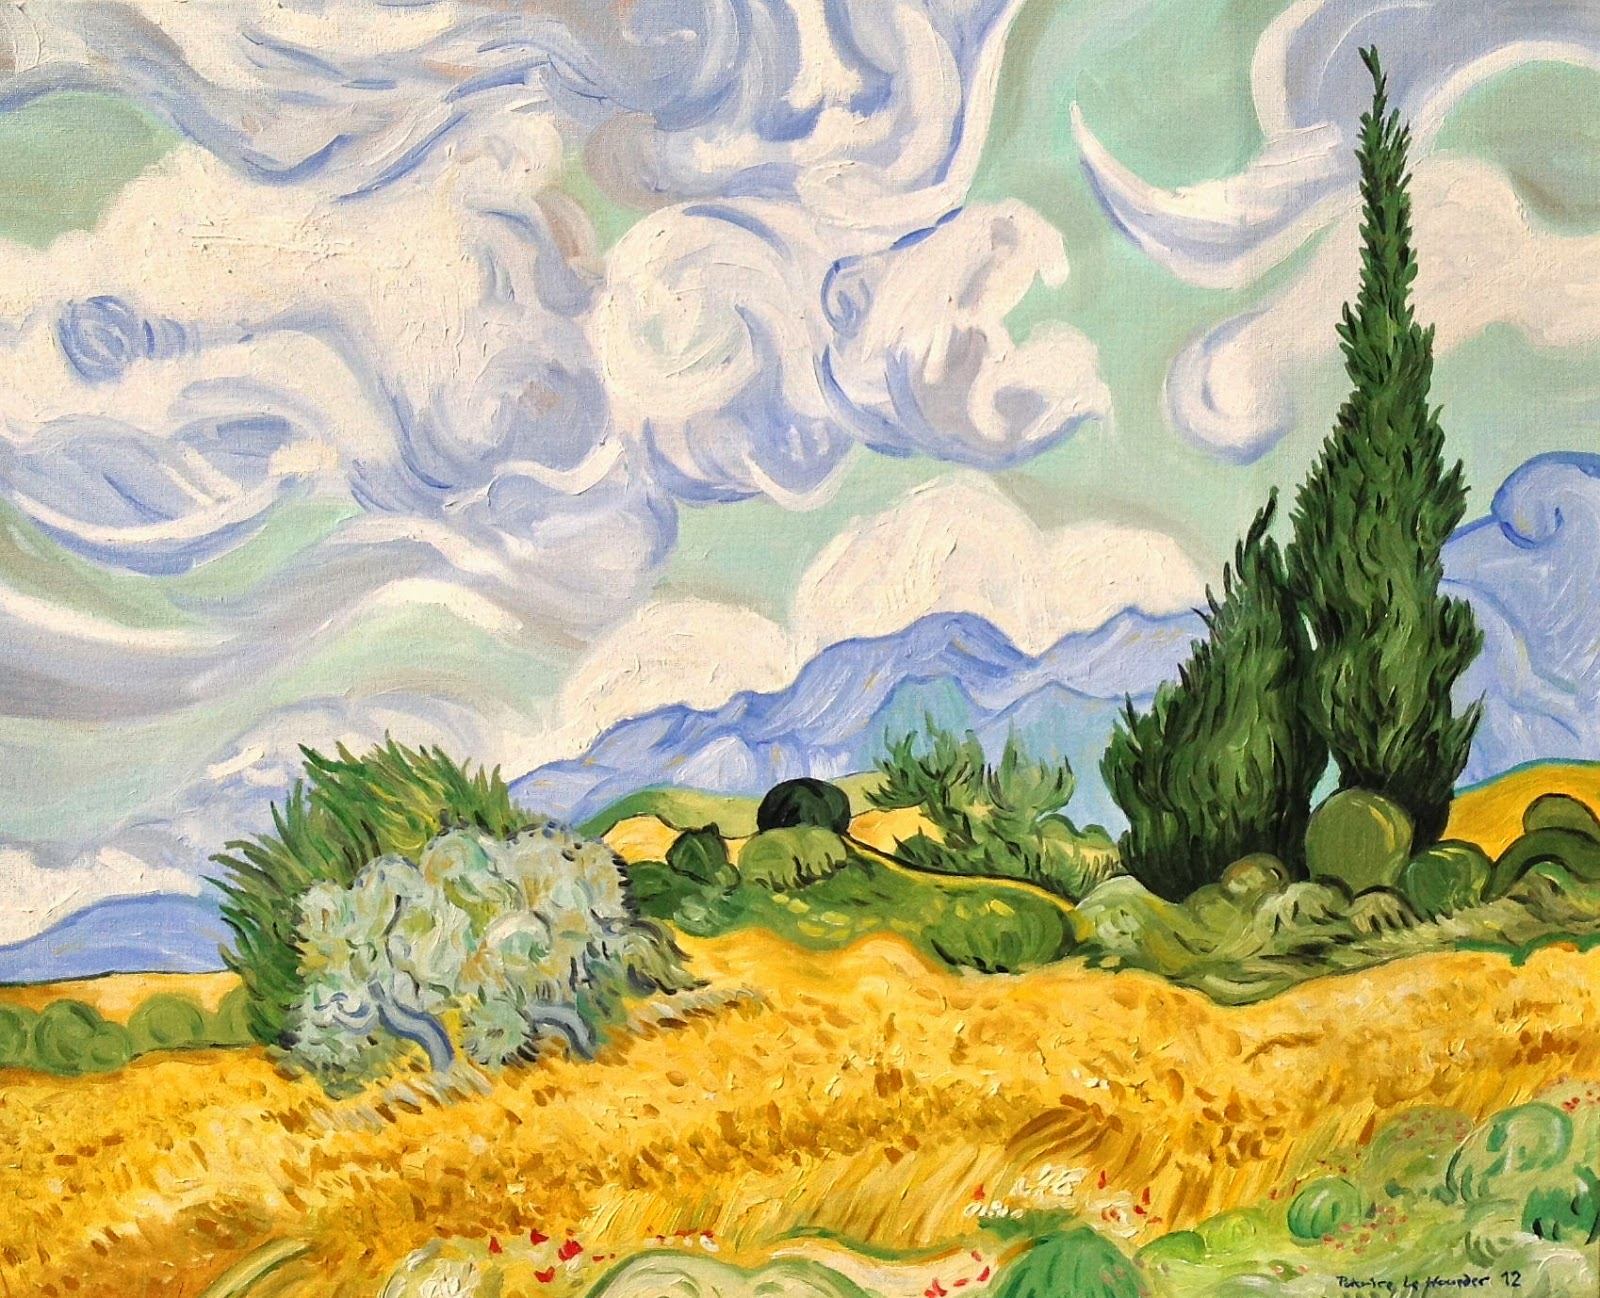
\includegraphics[scale=1.25]{v}}} % Image background
\centering
\vspace*{5cm}
\par\normalfont\fontsize{35}{35}\sffamily\selectfont
\textbf{Matematik 3 \\ Noter }\\
{\LARGE }\par % Book title
\vspace*{1cm}
{\Huge Martin Sung Jensen}\par % Author name
\endgroup

%----------------------------------------------------------------------------------------
%	COPYRIGHT PAGE
%----------------------------------------------------------------------------------------

\newpage
~\vfill
\thispagestyle{empty}

%\noindent Copyright \copyright\ 2014 Andrea Hidalgo\\ % Copyright notice

\noindent \textsc{Matematik 3, Aalborg universitet}\\



\noindent \textit{2015} % Printing/edition date

%----------------------------------------------------------------------------------------
%	TABLE OF CONTENTS
%----------------------------------------------------------------------------------------

\chapterimage{lol.jpg} % heading image

\pagestyle{empty} % No headers

\renewcommand\contentsname{Indholdsfortegnelse}
\renewcommand{\bibname}{Litteratur}
\tableofcontents% Print the table of contents itself

%\cleardoublepage % Forces the first chapter to start on an odd page so it's on the right

\pagestyle{fancy} % Print headers again

%----------------------------------------------------------------------------------------
%	CHAPTER 1
%----------------------------------------------------------------------------------------

\chapterimage{lol.jpg} % Chapter heading image

\chapter{Laplace transformation}
\section{Partiel integration}
\begin{equation}
\int f(x)g(x)dx=F(x)\cdot g(x)-\int F(x) \cdot g'(x)dx
\end{equation}
eller
\begin{equation}
\int f'(x)g(x)dx=f(x)\cdot g(x)-\int f(x) \cdot g'(x)dx
\end{equation}
eller
\begin{equation}
\int_{a}^{b}f(x)g(x)dx=[f(x)G(x)]_{a}^{b}-\int_{a}^{b}f'(x)G(x)dx
\end{equation}

\section{Blandede Laplace transformation}
\subsection{Eksempel 1 opg. 6.1(1)}
Find transformationen til $2t+8$. Antag at $a, b, \omega, \theta$ er konstanter.\\\\
svar:\\
\begin{equation}
\mathfrak{L}(2t+8)=\mathfrak{L}(2t)+\mathfrak{L}(8)=2\mathfrak{L(t)}+8\mathfrak{L}(1)
\end{equation}
1 og t kan slåes op i tabel 6,1. Svaret er dermed:
\begin{equation}
\frac{2}{s^2}+\frac{8}{s}
\end{equation}

\subsection{Eksempel 2  opg. 6.1(3) }
Find transformationen til $cos2 \pi t$. Antag at $a, b, \omega, \theta$ er konstanter.\\\\
svar:\\
\begin{equation}
\mathfrak{L}(cos2\pi t)=\frac{s}{s^2+4\pi^2}
\end{equation}

\subsection{Eksempel 3 opg. 6.1(10)}
Find transformationen til figuren. Antag at $a, b, \omega, \theta$ er konstanter.\\\\

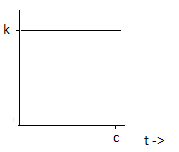
\includegraphics[scale=1]{kkk.png}\\
svar:\\
Vi har k på y-aksen og t på x-aksen. Derfor er funktionsværdien som den er.

\begin{equation}
\begin{split}
\mathfrak{L}(f(t)) & =\int_{0}^{\infty}e^{-st}dt\\
& = \int_{0}^{c}ke^{-st}dt
& = [\frac{ke^{-st}}{s}]^c_0 
& = \frac{k}{s}(1-e^{-sc})
\end{split}
\end{equation}



\subsection{Eksempel 4 opg. 6.1(11)} \label{juksi}
Find transformationen til figuren. Antag at $a, b, \omega, \theta$ er konstanter.\\\\

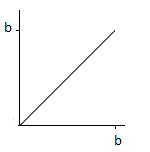
\includegraphics[scale=1]{bbb.png}\\
svar:\\
\begin{equation}
\begin{split}
\mathfrak{L}(f(t)) &= \int_{0}^{\infty}te^{-st}dt\\
& =\int_{0}^{b}te^{-st}dt\\
& = [-\frac{t}{s}e^{-st}]^b_0+\frac{1}{s}\int_{0}^{b}e^{-st}dt\\
& = -\frac{b}{s}e^{-sb}[\frac{1}{s^2}e^{-st}]^b_0\\
& = - \frac{b}{s}e^{-sb}- \frac{1}{s^2}e^{-sb}+ \frac{1}{s^2}\\
& = \frac{1}{s^2}-(\frac{b}{s}+\frac{1}{s^2})e^{-sb}
\end{split}
\end{equation}

\subsection{Eksempel 5 opg. 6.1(16)}
Find transformationen til figuren. Antag at $a, b, \omega, \theta$ er konstanter.\\\\

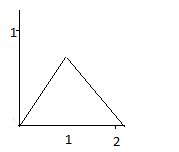
\includegraphics[scale=1]{12.png}\\
Svar:\\
Man skal dele figuren i to. Første del er lavet i \ref{juksi}. Fra 1 til 2 skal man lade som at stregen går fra 2 på y aksen og ned. Til sidst lægges de to resultater sammen.
\begin{equation}
\begin{split}
\mathfrak{L}(f(t)) &= \int_{1}^{2}e^{-st}dt\\
& = [(2-t)\frac{1}{-s}e^{-st}]^2_1-\frac{1}{s}[\frac{1}{
-s}e^{-st}]^2_1 \\
& = 0- \frac{1}{-s}e^{-s}+[\frac{1}{s^2}e^{-st}]^2_1 \\
& = \frac{1}{s}e^{-s}+(\frac{1}{s^2}e^{-s2}-\frac{1}{s^2}e^{-s})\\
1. del + ovenstaaende=\frac{2e^{-s}-e^{-2}-1}{s^2}
\end{split}
\end{equation}


\section{ODE eksempler - Begyndelsesværdiproblemer}

\subsection{Eksempel 1 opg. 6.2(4)}
Løs begyndelsesværdiproblemet  med Laplacetransformation for følgende:
\begin{equation}
y''+9y=10e^{-t}, \hspace{1cm} y(0)=0, y'(0)=0
\end{equation}
svar:\\
Dette kan skrives på følgende facon:
\begin{equation}
\mathfrak{L}[y'']+9\mathfrak{L}[y]=10\mathfrak{L}[e^{-t}]
\end{equation}
Her skal vi benytte følgende:
\begin{theorem} \label{teori1}
\begin{equation}
\mathfrak{L}(f')=s\mathfrak{L}(f)-f(0)
\end{equation}
\begin{equation}
\mathfrak{L}(f'')=s^2 \mathfrak{L}(f)-\textcolor{red}{s}f(0)-f'(0)
\end{equation}
\end{theorem}
Vi indsætter de to formler fra theorem \ref{teori1}. Husk at benytte infoen om startværdierne, altså y(0)=0 osv. Vi får følgende: (bemærk at $a=-1$ da der står $-t$)
\begin{equation}
\begin{split}
s^2\cdot Y(s)-s\cdot 0 - 0 +9(Y(s))  =10 \cdot \frac{1}{s+1}&  \Updownarrow\\
 s^2Y(s)+9Y(s)=\frac{10}{s+1}& \Updownarrow\\
 (s^2+9)Y(s)=\frac{10}{s+1} & \Updownarrow\\
 Y(s)= \frac{10}{(s+1)(s^2+9)}
\end{split}
\end{equation}
Nu skal vi dekomponere højresiden. Man kan dele Bs+c op i to, hvis det er. Husk s!
\begin{equation}\label{haha}
\frac{10}{(s+1)(s^2+9)}=\frac{A}{(s+1)}+\frac{Bs+C}{S^2+9}
\end{equation}
Nu dividerer vi elementerne fra nævneren en for en indtil at 10 står alene. Husk at dividere på hvert led på højresiden. Hvis vi gør dette får vi følgende:
\begin{equation}\label{husks}
10=A(s^2+9)+(Bs+C)(s+1)
\end{equation}
I \ref{haha} kan vi se at -1 er en rod til A.  Og derfor siger vi $A((-1)^2+9)=10 \Rightarrow A=1$ \\\\
Nu skal vi finde C, og dette gør vi ved at vælge et tal vi ikke har brugt før. Dette kunne f.eks. være 0. Dette sætter vi ind på s'ets plads i \ref{husks}.\\
$s=0$
\begin{equation}
\begin{split}
10=1(0^2+9)+(0B+C)(s+1) & \Updownarrow \\
10= 9+c & \updownarrow \\
c=1
\end{split}
\end{equation}
B finder vi på samme måde. Husk ikke at glemme s i Bs! Her bruger vi $s=2$.
\begin{equation}
\begin{split}
10=1 \cdot 13 + (1+2b)(3) & \Updownarrow \\
10 = 13 +3 +6B & \Updownarrow \\
B=-1
\end{split}
\end{equation}
Nu kan vi indsætte 1,1 og -1, så vi får følgende:
\begin{equation}
\frac{1}{s+1}+\frac{-s+1}{s^2+9}
\end{equation}
Dette kan også skrives som:
\begin{equation}
\frac{1}{s+1}+\frac{-s}{s^2+9}+\frac{1}{s^2+9}
\end{equation}
Vi Kigger i tabellen og ser at det giver:
\begin{equation}
e^{-t}-cos(3t)+\frac{1}{3}sin(t)
\end{equation}

\subsection{Eksempel 1 opg. 6.2(1)}
Løs begyndelsesværdiproblemet  med Laplacetransformation for følgende:
\begin{equation}
y'+\frac{2}{3}y=-4cos(2t), \hspace{1cm} y(0)=0
\end{equation}
Vi benytter os af theorem \ref{teori1} og vi husker at y(0)=0.
\begin{equation}
sY(s)+\frac{2}{3}Y(s)=-4(\frac{s}{s^2+2^2}
\end{equation}
Vi skal have Y(s) til at stå alene:
\begin{equation}
\begin{split}
Y(s)(s+\frac{2}{3})=\frac{-4s}{s^2+2^2} & \Updownarrow \\
Y(s)=\frac{-4s}{(s^2+2^2)(s+\frac{2}{3}}
\end{split}
\end{equation}
Vi dekomponerer igen. Vi ser at en rod er $-\frac{2}{3}$
\begin{equation}
\frac{-4s}{s^2+s^2(s+\frac{2}{3}}=\frac{A}{s+\frac{2}{3}}+\frac{Bs+c}{s^2+2^2}
\end{equation}
Vi sætter vores rod $-\frac{2}{3}$ ind i "a-delens" stykke.

\begin{equation}
\begin{split}
-4s=a(s^2+s^2) & \Updownarrow \\
-4s=a((\frac{2}{3})^2+4) & \Updownarrow \\
-4s=a(\frac{4}{9} + 4) & \updownarrow \\
a=\frac{3}{5}
\end{split}
\end{equation}
Nu finder vi først c og derefter b.\\
$s=0$
\begin{equation}
\begin{split}
-4s=\frac{3}{5}(0+2^2)+c(\frac{2}{3}) & \Updownarrow \\
c=-\frac{18}{5}
\end{split}
\end{equation}
til b brugern vi $s=2$
\begin{equation}
\begin{split}
-4s=\frac{3}{5}(8)+(2b+ \frac{18}{5})(2+\frac{2}{3}) & \Updownarrow \\
b=- \frac{3}{5}
\end{split}
\end{equation}
Nu kan vi indsætte a,b og c på deres pladser, så vi får følgende brøker:
\begin{equation}
\frac{\frac{3}{5}}{s+ \frac{2}{3}}+ \frac{\frac{-3}{5}s}{s^2+2^2}+\frac{\frac{-18}{5}}{s^2+2^2}
\end{equation}
Nu skal vi bare få det til at ligne noget fra tabellen. Dette kan gøres ved at trække tælleren ned.

\subsection{Dekomponering eksempel 1}
$ds+e$ er placeret over $s^2+1$ fordi at det ikke umiddelbart lader sig gøre at finde roden.
\begin{equation}
\frac{60}{(s+1)(s-1)(s+2)(s^2+1)}=\frac{a}{s+1}+\frac{b}{s-1}+\frac{c}{s+2}+\frac{ds+e}{s^2+1}
\end{equation}
Ved at multiplicere ligningen med fællesnævneren fås:
\begin{equation}
60=a(s-1)(s+2)(s^2+1)+b(s+1)(s+2)(s^2+1)+c(s+1)(s-1)(s^2+1)
\end{equation}
\begin{equation}
60=a(s-1)(s+2)(s^2+1)+b(s+1)(s+2)(s^2+1)+c(s+1)(s-1)(s^2+1)+(ds+e)(s+1)(s-1)(s+2)
\end{equation}
Indsættes rødderne $s=-1$ , $s=1$ , $s=-2$ , fås:\\
s=-1
\begin{equation}
60=a(-1-1)(-1+2((-1)^2+1)\Leftrightarrow a=-15
\end{equation}
s=1
\begin{equation}
60=b(1+1)(1+2)(1^2+1)\Leftrightarrow b=5
\end{equation}
s=-2
\begin{equation}
60=c(-2+1)(-2-1)((-2)^2+1)\Leftrightarrow c=4
\end{equation}
For at bestemme d og e indsættes to små hele tal, som ikke tidligere har været indsat, f. eks. $s=0$ og $s=2$\\
s=0:
\begin{equation}
60=-15(-1)\cdot2\cdot1+5\cdot2\cdot1+4\cdot1(-1)\cdot1+e\cdot1(-1)2\Leftrightarrow e=-12
\end{equation}
s=2:
\begin{equation}
60=-15\cdot1\cdot4\cdot5+5\cdot3\cdot4\cdot5+4\cdot3\cdot1\cdot5+(2d-12)\cdot3\cdot1\cdot4 \Leftrightarrow d=6
\end{equation}
Vi har altså:
\begin{equation}
Y(s)=\frac{-15}{s+1}+\frac{5}{s-1}+\frac{4}{s+2}+\frac{6s-12}{s^2+1}+\frac{1}{s+2}=\frac{-15}{s+1}+\frac{5}{s-1}+\frac{5}{s+2}+\frac{6s-12}{s^2+1}
\end{equation}
Nu kan man bruge en tabel til at finde løsningen :)

\subsection{Dekomponering eksempel 2}
Hvis brøken er "uægte" laves denne om til en "ægte" brøk vha. polynomiedivision\footnote{Man placerer næveren til venstre for brøken. Derefter divideres den højeste værdi på venstresiden med den højeste på h.siden. Resultatet skriven ovenover højresiden. Nu ganges værdierne, en for en, fra venstresiden med det tal der står øverst. Resultatet trækkes fra h.siden. Husk ikke at bruge tallene flere gange. Resultatet er det der står i toppen + din rest over venstresiden.} Hvis tællerens grad er større eller lig med nævnerens grad er brøken  "uægte".\\
Her er en ægte brøk:
\begin{equation}
\frac{5x^2-9x+2}{x^3-4x^2+6x-4}
\end{equation}
Dette kan omskrives til:
\begin{equation}
\frac{5x^2-9x+2}{(x-2)(x^2-2x+2)}
\end{equation}
hvor nævneren er skrevet som et produkt af de simplest mulig reelle polynomier (dvs.reelle polynomier af første grad og reelle polynomier af anden grad med negativ diskriminant.\\\\
Ved at betragte nævnerens faktorer ses nu, at den simpleste omskrivning til en sum af ægte brøker må være af formen:
\begin{equation}\label{bax}
\frac{5x^2-9x+2}{(x-2)(x^2-2x+2)}=\frac{a}{x-2}+\frac{bx+c}{x^2-2x+2}
\end{equation}
hvor a, b og c er konstanter. $bx+c$ kan også opdeles i en $bx$ og $c$ brøk.\\\\
Konstanten a findes ved at multiplicere ligning \ref{bax} med den til \textit{a} hørende nævner. Altså vi ganger med $x-2$ på begge sider af lighedstegnet og i alle led.
\begin{equation}
\frac{5x^2-9x+2}{x^2-2x+2}=a+(x-2)\frac{bx+c}{x^2-2x+2}
\end{equation}
og derpå indsætte $x=2$ så \textit{a} står alene på højre side:
\begin{equation}
\frac{5x^2-9\cdot2+2}{2^2-4+2}=a+0\Leftrightarrow a=\frac{4}{2}\Leftrightarrow a=2
\end{equation}
For at finde \textit{b} og \textit{c} indsættes 2 små hele tal, som ikke tidligere har været indsat(indsættes i ligning \ref{bax} hvor også a er indsat):\\\\
$x=0$
\begin{equation}
\frac{2}{(-2)(2)}= \frac{2}{-2}+\frac{c}{2}\Leftrightarrow -\frac{1}{2}=-1+\frac{c}{2} \Leftrightarrow c=1
\end{equation}
$x=1$ 
\begin{equation}
\frac{5-9+2}{(1-2)(1-2+2)}=\frac{2}{1-2}+\frac{b+1}{1-2+2}\Leftrightarrow 2=-2+b+1 \Leftrightarrow b=3
\end{equation}
Vi har hermed fundet:
\begin{equation}
\frac{5x^2-9x+2}{x^3-4x^2+6x-4}=\frac{2}{x-2}+\frac{3x+1}{x^2-2x+2}
\end{equation}

\section{Unit step funktionen (Heaviside funktionen) og 2. shift (t-shifting)}

\subsection{Eksempel 1 opg. 6.3(3)}
Skitser $t-3(t>3)$, som antages at være 0 uden for det givne interval. Vis transformationen vha. af unit step funktioner. \\\\
svar:\\
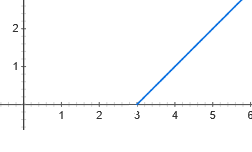
\includegraphics[scale=1]{63.png}\\
\begin{equation}
f(t)=\begin{Bmatrix}
0 & , t<3 \\ 
 t-3 & , t>3 
\end{Bmatrix}
\end{equation}
Her benytter vi os af unit step funktionen som er:
\begin{equation}
(t-a)=\begin{Bmatrix}
0 & , t<a \\ 
1 & , t>a
\end{Bmatrix}
\end{equation}
Så vi kan skrive $u(t-3)g(t-3)$. Ifølge theorem 1(s. 219) har vi:
\begin{equation}
\mathfrak{L} \{ f(t)\} =\mathfrak{L} \{ u(t-3)g(t-3)  \}=e^{-3s} G(s)
\end{equation}
Hvis man kigger i tabel 6.1  ses det at $G(s)=\frac{1}{s^2}$. Det er t der skal slåes op, da dette angiver funktionsværdien. Et stort bogstav med s indeni angiver at vi skal slå værdien op.\\\\
Så derfor er svaret:
\begin{equation}
\mathfrak{L} \{ f(t) \} = \frac{e^{3s}}{s^2}
\end{equation}

\subsection{Eksempel 2 opg. 6.3(7)} \label{jojojo}
Skitser $e^{(\pi / 2)t}$, som antages at være 0 uden for det givne interval. Vis transformationen vha. af unit step funktioner. \\\\
svar:\\
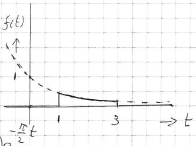
\includegraphics[scale=1]{snip.PNG}\\
Her ser vi at den starter på 1 og slutter på 3.  For mere info se på s. 218-220 i bogen. Vi kan opstile følgende:
\begin{equation}
e^{(-\frac{\pi}{2})t}(u(t-1)-u(t-3))
\end{equation}
Nu vil det være smart at få t-1 og t-3 som eksponter. Så får vi:
\begin{equation}
f(t)=u(t-1)e^{\frac{-\pi}{2}(t-1)}\cdot e^\frac{-\pi}{2}-u(t-3)e^{\frac{-\pi}{2}(t-3)} \cdot e^{\frac{-3\pi}{2}}
\end{equation}
Eksponenterne svarer til $f(t-a)$ på s. 219 i theorem 1. Altså f er $e^{\frac{\pi}{2}}$ og $(t-a)$ svarer til $t-1$ som er i vores eksponent.
$u(t-a)$  laver vi om til $\frac{e^{-as}}{s}$ (se. s. 218) - a er selvfølgelig 1 og 3 i dette tilfælde.\\\\
For at komme frem til $t-1$ og $t-3$ i eksponenterne benytter vi at $e^a \cdot e^b = e^{a+b}$ og vi udnytter også at $e^{-\frac{\pi}{2}} + e^{\frac{\pi}{2}} = 1$...og man må jo gerne gange med 1. Del. Husk at se på \ref{jojojo} i to dele. Så er det nemmere. \\
Så resultatet er:
\begin{equation}
\frac{e^{-s -\frac{1}{2}\pi}-e^{-3s -\frac{3\pi}{2}}} {s+\frac{\pi}{2}}
\end{equation}

\section{Diracs deltafunktion}
\subsection{Eksempel 1 opg. 6.4(3)}
Find og skitser løsningen til følgende:
\begin{equation}
y''+9y= \delta (t- \frac{\pi}{2}) , \hspace{1cm} y(0) =2, y'(0)=0
\end{equation}
Her udnytter vi at $ \mathfrak{L} \{  \delta (t-a)\}=e^{-as}$.\\
Vi Laplacetransformerer og vi husker at ALLE s'er.
\begin{equation}
\begin{split}
s^2Y(s)-S(y(0)-Y'(0)+9Y(s) & =e^{-\frac{1}{2} \cdot \pi s}\\
s^2Y(s)-2-0+9Y(s)=e^{\frac{1}{2}-\pi s}\\
Y(s)(s^2+9) &=e^{-\pi s}+2s \\
Y(s) &=\frac{e^{-\pi s}}{s^2+9}+\frac{2s}{s^2+9}
\end{split}
\end{equation}
Vi vil forsøge at få det til at ligne noget fra tabel 6.1. Vi sætter $\omega=3$ og vi husker at $\omega$ skal være den samme værdi i både cos og sin. Det er derfor at vi ganger $\frac{1}{3}$ på sin.
\begin{equation}
Y(s)=\frac{\omega}{s^2+\omega^2}\frac{1}{3}e^{-\frac{1}{2}\pi s}+ 2\frac{s}{s^2+ \omega^2}
\end{equation}
Her har vi udnyttet at $f(t-a)=e^{-as}F(s)$ . Så derfor kommer det der var i eksponenten ind i sinus.
\begin{equation}
y(t)=sin\omega (t- \frac{1}{2} \pi)+2cos \omega t
\end{equation}
Altså $e^{\frac{1}{2} \pi s}$ er der vi bruger time-shift.


\chapter{Fourier rækker og transformationer}
\section{Perioder og fundementale perioder}

\subsection{Eksempel 1 opg. 11(1)}
Den \textit{fundementale periode} er den mindste positive periode. Find den for:\\
\begin{table}[hts!]
\centering
\caption{Fundementale perioder}
\label{adadads}
\begin{tabular}{|l|l|l|l|l|l|l|l|l|}
\hline
Find    & cos x  & sin x  & cos 2x & sin 2x & cos $\pi x$ & sin $\pi x$ & cos 2$\pi x$ & sin 2$\pi x$ \\ \hline
Periode & 2$\pi$ & 2$\pi$ & $\pi$  & $\pi$  & 2           & 2           & 1            & 1            \\ \hline
\end{tabular}
\end{table}

En periode er på $2\pi$ og derfor skal $2 \pi$ divideres med det der står foran x. sin 3x betyder at den svinger 3 gange på en periode. For mere info se s. 475

\subsection{Eksempel 2 opg. 11(2)}
Den \textit{fundementale periode} er den mindste positive periode. Find den for:\\
\begin{table}[hts!]
\centering
\caption{Fundementale perioder}
\label{my-label}
\begin{tabular}{|l|l|l|l|l|l|l|}
\hline
Find    & cos nx            & sin nx            & cos $\frac{2 \pi x  }{k}$ & sin $\frac{2 \pi x,}{k}$ & cos $\frac{2 \pi nx,}{k}$ & sin $\frac{2 \pi nx,}{k}$ \\ \hline
Periode & $\frac{2 \pi}{n}$ & $\frac{2 \pi}{n}$ & k                        & k                       & $\frac{k}{n}$            & 2                        \\ \hline
\end{tabular}
\end{table}
Princippet er det samme som i tabel \ref{adadads}
\subsection{Eksempel 3 opg. 11(3)}
Hvis $f(X)$ og $g(x)$ har samme periode $p$, vis at  $h(x)=af(x)+bg(x)(a,b,konstanter)$ har perioden p. Således at alle funktioner af perioden laver et vektorrum.\\
\begin{equation}
\begin{split}
f(x+p) &= f(x)\\
g(x+p)&=g(x)\\
h(x) &= af(x)+bg(x)\\
Bevis\\
h(x+p)&=af(x+p)+bg(x+p)\\
&= af(x)+bg(x)\\
&= h(x)
\end{split}
\end{equation}

\subsection{Eksempel 4 opg. 11(4)}
Hvis $f(x)$ har perioden p, vis $f(ax),a\neq 0$ og $f(\frac{x}{b}),b \neq 0$ er periodiske funktioner af x af periode $p/a$ og $bp$.\\
svar:\\
Alt sker en faktor a hurtigere. Det er det samme som at sige at perioden bliver a mindre\\\\
Iforhold til b  så sker alt langsommere, fordi vi dividerer b på. Så hvis nu b er 2. Så skal vi dividere perioden med 2, altså alt går langsommere!
\subsection{Eksempel 5 opg. 11(5)}
Vis at $f=konstant$ er periodisk med en hvilken som  helst periode.\\
svar:\\\\
$f(x)=f(x+p)$\\
se side 475
\newpage
\subsection{Eksempel 6 opg. 11(6-10)}
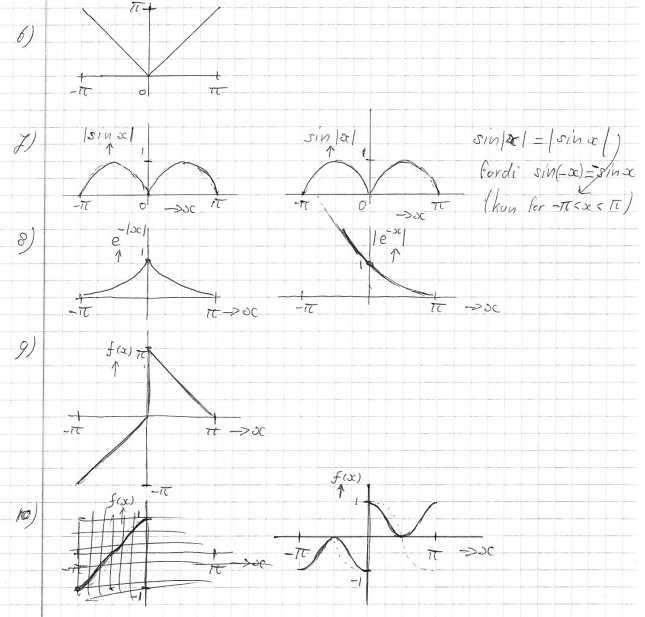
\includegraphics[scale=1]{grafer.PNG}\\
\subsection{Eksempel 6 opg. 11(11)}
Benyt integration ved substition til at integrere $cos(nx)$\\
svar:
\begin{equation}
t = nx\\
\frac{dt}{dx} =n\\
dx =\frac{1}{n}dt
\end{equation}
Så integrerer vi bare cos uden at tage hensyn til hvad der står  i parentesen. Derefter ganger vi dx på og til sidst putter vi t ind igen. 
\begin{equation}
\int{ cos} dx=\frac{sin(nx)}{n}
\end{equation}
\section{Fourier serier}
\subsection{Eksempel 1 opg. 11(12)}
Find fourierserien af $f(x)=\mid x \mid$, som har perioden $2 \pi$ . Derudover skitser den.\\
svar:\\\\
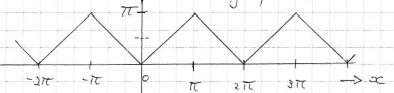
\includegraphics[scale=1]{topi.PNG}\\
Det vi skal finde er:
\begin{equation}
f(x)=a_0+\sum_{n=1}^{\infty} (a_n cos(nx)+b_n sin(nx))
\end{equation}
Vi starter først med at finde $a_0$
\begin{equation}
a_0=\frac{1}{2 \pi}\int_{-\pi}^{pi}f(x)dx
\end{equation}
Vi ser at fra $-\pi$ til 0 der falder den med x og derfor kan vi skrive følgende:
\begin{equation}
\begin{split}
a_0 &=\frac{1}{2 \pi}\int_{-\pi}^{0}-x\quad dx \quad +\quad \frac{1}{2 \pi}\int_{0}^{\pi}x\quad dx\\
&=\frac{1}{2 \pi}\left [-\frac{1}{2}x^2\right ]_{-\pi}^0+ \frac{1}{2 \pi}
\left [  \frac{1}{2}x^2\right ]_0^\pi \\
&=\frac{1}{2\pi}(0-(-\frac{1}{2}(-\pi)^2)+\frac{1}{2\pi}(\frac{1}{2}\pi^2-0)\\
&= \frac{1}{2\pi}(\frac{2\pi^2}{2})\\
&= \frac{1}{2}\pi
\end{split}
\end{equation}
Det er vigtigt at huske at $(-a)^2$ ALTID giver $a^2$\\\\
Nu skal vi finde:
\begin{equation}
a_n=\frac{1}{\pi}\int_{-\pi}^{\pi}f(x)cos(nx)\quad dx
\end{equation}
Her skal vi benytte os af integration ved substition og partiel integration.
\begin{equation}\label{jodis}
\begin{split}
a_n&=\frac{1}{\pi}\int_{-\pi}^{\pi} \mid x \mid cos(nx)\quad dx\\
&= \frac{1}{\pi}\int_{-\pi}^{0}-xcos(nx)\quad dx\quad+\quad\frac{1}{\pi}\int_{0}^{\pi}xcos(nx)\quad dx\\
\end{split}
\end{equation}
Her benytter vi os integration ved substition.
\begin{equation}
t=nx\\
\frac{dt}{dx}=n\\
dx=\frac{1}{n}dt
\end{equation}
Vi fortsætter fra \ref{jodis} og vi starter med at tage fra $\int_{-\pi}^{0}$
\begin{equation}
\begin{split}
&=  \frac{1}{\pi}(\left [ \frac{sin(nx)}{n} \cdot (-x) \right]_{-\pi}^0-\int_{-\pi}^{0}\frac{sin(nx)}{n} \cdot (-1)\quad dx)\\
&= \frac{1}{\pi}(0- \frac{1}{n^2}\left[cos(nx) \right]_{-\pi}^{0})\\
&=\frac{1}{\pi}(-\frac{1}{n^2}(1-cos(n \pi))\\
&= \frac{1}{\pi}(\frac{cos(n \pi)-1}{n^2})\\
&= \frac{cos(n \pi)-1}{\pi n^2}
\end{split}
\end{equation}
Vi ser at -$pi$ er det samme som $\pi$ det kommer bare an på hvilken vej man drejer rundt. Vi lægger også mærke til at i anden del. der er -x skiftet ud med x!
\begin{equation}\label{koekoe}
\begin{split}
&= \frac{1}{\pi}(0-\frac{1}{n^2}\left [-cos(nx) \right ]_0^{\pi} )\\
&= \frac{1}{\pi}(-\frac{1}{n^2}(-cos(n \pi)-(-1))\\
&= \frac{cos(n \pi)-1}{\pi n^2}
\end{split}
\end{equation}
Det betyder at vi kan lægge de to sammen så det bliver til $\frac{2cos( \pi n )-2}{\pi n^2}$. Det vil sige at $a_n=\frac{-4}{\pi n^2}$  ved ulige tal\\
Nu udregnes $b_n=\frac{1}{\pi}\int_{-\pi}^{\pi}f(x)sin(nx) dx=0$\\
Vi husker at $a_0$ er gennemsnitsværdien! (offset) og resultatet er:\\
\begin{equation}
f(x)=\frac{1}{2}\pi+\sum_{n=1}^{\infty}\frac{-4}{\pi (2n-1)^2}\cdot cos((2m-1)x)
\end{equation}
Man kunne også have brugt udtrykket efter \ref{koekoe}, men den ovenstående måde at skrive det op på, skyldes at den kun tager ulige tal med!!(smart)

\subsection{Eksempel 6 opg. 11(13)}
Find fourierserien for: $f(x)=\begin{pmatrix}
x & if &-\pi<0 \\ 
 \pi-x&if  & 0<x<\pi
\end{pmatrix}$ . Perioden er $2 \pi $\\
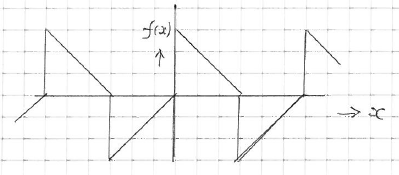
\includegraphics[scale=1]{takker.PNG}\\
ed at kigge på figuren ses det at gennemsnittet er 0! Derfor siger vi $a_0=0$ \\
$a_n$ udregnes. Først finder vi $\int_{- \pi}^0$
\begin{equation}
\begin{split}
a_0 &=\frac{1}{\pi}\int_{- \pi}^{0}xcos(nx)\quad dx \quad + \frac{1}{\pi}-cos(nx)\quad dx\\
&=\frac{1}{\pi}( \left [  \frac{sin(nx)x}{n}   \right ]_{- \pi}^0-
\end{split}
\end{equation}

% ----------------------------------------------------------------------------------------
% 	BIBLIOGRAPHY
% ----------------------------------------------------------------------------------------

\begin{thebibliography}{9}


          

     



\end{thebibliography}


   




\end{document}